\section{Xây dựng đội hình}
Sau khi thực hiện xong pha khám phá để có được các thông tin cần thiết của vật, hệ thống sẽ chuyển sang thực hiện pha đẩy vật nhằm di chuyển vật tới vị trí mong muốn. Với hệ thống được xây dựng để điều khiển theo lực, các cấu hình khác nhau sẽ liên tục được xây dựng dựa theo wrench mong muốn và chuyển đổi mỗi khi cần thiết. Phần này sẽ trình bày mô hình hóa bài toán đội hình, thước đo đánh giá độ ổn định của cấu hình và bài toán tối ưu được xây dựng.
\subsection{Mô hình hóa bài toán xây dựng đội hình}
Trong một hệ có $n$ robot, với một wrench điều khiển mong muốn $w_d = [f_{\text{x,d}} \, f_{\text{y,d}} \, \tau_d ]$, bài toán đặt ra là cần tìm một cấu hình $u = [u_1 \ldots u_n]^T$ với $u_i \in U, i \in N$ sao cho khi mỗi robot tác dụng lực đẩy vuông góc so với cạnh tương ứng trong khoảng $[0, f_{\text{max}}]$ tại từ vị trí trong $u$, tổng hợp wrench lên khối tâm của vật là có thể đạt được $w_d$, đồng thời thoả mãn các điều kiện về an toàn và có độ ổn định cao với thước đo được xây dựng trước. Nói cách khác, ta coi bài toán tìm đội hình cho $n$ robot như một bài toán tìm grasp tốt nhất cho $n$ điểm tiếp xúc. Mỗi robot sẽ tự giải ra bộ vị trí $u$ này độc lập, sao cho tất cả robot đều trả về chung một cấu hình, sau đó bằng một cơ chế thảo luận và phân nhiệm, mỗi robot sẽ tự nhận thức được vị trí của bản thân trong cấu hình mà không bị trùng lặp với robot khác.

Với mỗi vị trí $u_i$, vector pháp tuyến với cạnh tại vị trí tương ứng là $n_i = n(u_i) \in R^2$, với , cánh tay đòn $r_i = lv(u_i)$ đến khối tâm của vật có thể được xác định. Khi đó, ánh xạ grasp map được xác định bởi công thức :
\begin{equation}
    G(u) =
    \begin{bmatrix} n(u_1)\; \cdots\; n(u_n) \\
        lv(u_1)\; \cdots\; lv(u_n)
    \end{bmatrix}
    \in R^{3 \times N}
\label{eq:gmap2}
\end{equation}

Khi này, với lực đẩy của các robot $f_r = [f_1 \ldots f_n]$ với $f_i \in R, i \in R$ là lực đẩy của robot i, theo công thức \ref{eq:wrenchi} thì tổng hợp wrench tại khối tâm là:
\begin{equation}
    w_e = G(u)\,f_r
\label{eq:we}
\end{equation}


\subsection{Phương pháp đánh giá độ ổn định cấu hình}

Với một cấu hình $u$, ta xây dựng không gian làm việc $\mathcal{G}(u)$ của cấu hình trong không gian wrench. Không gian $\mathcal{G}(u)$ bao gồm tất cả các wrench có thể sinh ra tại khối tâm bằng khi ta thay đổi độ lớn các lực $f_i$ trong khoảng giới hạn, hay chính là grasp wrench space với các tiếp xúc tương ứng với cấu hình $u$. Vì khả năng thao tác riêng lẻ của robot i có thể được mô tả bởi đoạn thẳng $f_\text{max}\, gm(u_i)$, ta có thể xây dựng không gian $\mathcal{G}(u)$ bằng cách lấy tổng Minkowski của tất cả các đoạn thẳng này, trong đó $gm(u_i)$ tương ứng với cột thứ $i$ trong ma trận ánh xạ grasp map (\ref{eq:gmap2}).

\begin{figure}[H]
    \centering
    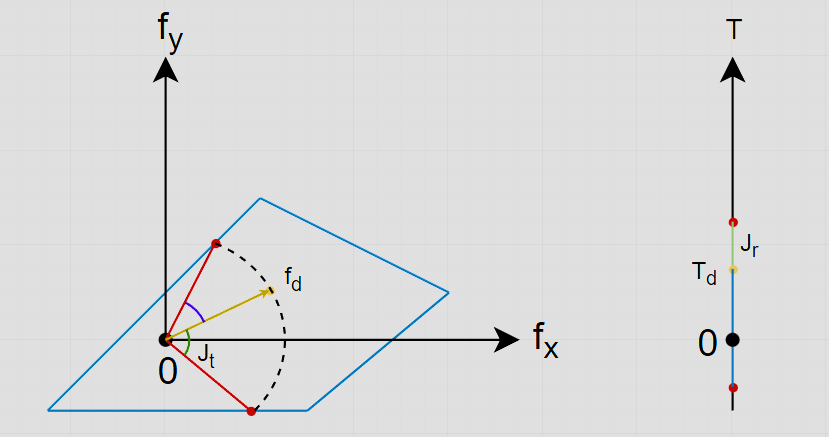
\includegraphics[scale=0.55]{chapter5/image/metric.png}
    \caption{Độ ổn định tịnh tiến $J_t$(trái) và xoay $J_r$(phải)}
    \label{fig:metric}
\end{figure}

Một cấu hình có thể được xem là khả thi khi $w_d \in \mathcal{G}(u)$, đây là điều kiện quan trọng nhất đảm bảo cấu hình có thể sinh ra lực mong muốn. Ngoài ra ta cũng mong muốn $w_d$ không nằm quá gần các mặt biên của $\mathcal{G}(u)$ nhằm nâng cao độ ổn định và gián tiếp giảm số lần tái cấu trúc cấu hình do vi phạm ràng buộc $w_d$ nằm ngoài $\mathcal{G}(u)$. Thước đo đánh giá độ ổn định của cấu hình được xây dựng theo nghiên cứu \cite{Rosenfelder2024}, tách riêng phần đánh giá ổn định quay và tịnh tiến thành hai phần riêng biệt. Trong đó, độ ổn định xoay $J_r$ được tính bằng cách lấy khoảng cách nhỏ nhất từ $w_d$ đến một trong hai đầu của đường thẳng $f = f_d = [f_{\text{x,d}} \, f_{\text{y,d}}]$ theo hướng mô men, đường thẳng này vuông góc với hình chiếu phẳng của $\mathcal{G}[u]$ tại  $\tau = \tau_d$. Giá trị này đại diện cho khả năng sinh ra các mô men gần với mô men mong muốn $\tau_d$ trong khi đang đồng thời sinh ra lực tịnh tiến $f_d$. Độ ổn định tính tiến $J_t$ có thể được tách ra thành hai thành phần con là độ ổn định về độ lớn của vector lực tịnh tiến và độ ổn định về chiều của vector lực tịnh tiến, trong đó độ ổn định về độ lớn thường không quá quan trọng, nên $J_t$ sẽ tập trung vào độ ổn định về chiều của vector lực. Xét hình chiếu của không gian làm việc $\mathcal{G}(u)$ tại mặt phẳng có mô men $\tau = \tau_d$, lấy giao điểm của đa giác thu được với một đường tròn có bán kính $|f_d|$, tâm tại gốc tọa độ. Lúc này $J_t$ được tính bằng góc nhỏ nhất giữa hướng lực mong muốn và các điểm giao này, tức là $J_t = \min\{\,|\alpha_1|,\; |\alpha_2|\,\}$. Giá trị này đại diện cho độ đa dạng về hướng quay của lực tác dụng có độ lớn $|f_d|$ trong không gian làm việc. Cách tính hai đại lượng $J_t$ và $J_r$ được thể hiện ở hình (\ref{fig:metric}).
\subsection{Xây dựng và giải bài toán tối ưu bằng ALPSO} 
Bài toán xây dựng đội hình được phát biểu dưới dạng một bài toán tối ưu hóa. Cụ thể, để giải quyết nhiệm vụ đặt ra, , các điều kiện cần thiết nhằm đẩy và xoay vật theo hướng mong muốn hiện tại được đưa vào dưới dạng các ràng buộc, trong khi các thuộc tính mong muốn được xét đến thông qua một hàm mục tiêu. Do đó bài toán cần giải có dạng: 
\begin{subequations}
\label{eq:op}
\begin{align}
\min_{u \in \mathbb{R}^N_{\ge 0}} \; J(u) = -c_1 J_t(u) - c_2 J_r(u)
\label{eq:op1} \\[4pt]
\exists\, \tilde{\mathbf{f}} \in \mathcal{F}
\quad \text{s.t.} \quad
G(u)\,\tilde{\mathbf{f}} = \mathbf{w}_d
\label{eq:op2} \\[4pt]
\mathrm{frD}(u_i, u_j) \ge d_{\min},
\qquad \forall i \neq j
\label{eq:op3}
\end{align}
\end{subequations}


trong đó $c_1$ và $c_2$ là các hệ số dương, $\mathrm{frD}$ là hàm tính khoảng cách giữa 2 vị trí trong cấu hình, $d_{\min} > r_r$ là khoảng cách an toàn tối thiểu giữa các robot trong hệ thống, đảm bảo rằng các robot không được bố trí quá gần nhau để tránh va chạm.

Để giải quyết nhiệm vụ đặt ra, điều quan trọng nhất là một đội hình phải thỏa mãn các ràng buộc \ref{eq:op2} và \ref{eq:op3}, trong đó \ref{eq:op2} đảm bảo tồn tại một bộ lực sinh ra bởi các robot cho cấu hình hiện tại sao tổng hợp wrench tại trọng tâm đúng bằng $w_d$, hay nói theo cách hình học là $w_d$ nằm trong không gian làm việc $\mathcal{G}(u)$, còn \ref{eq:op3} đảm bảo các robot không ở quá gần nhau. Hàm chi phí \ref{eq:op1} đánh giá mức độ tốt của cấu hình tương ứng xét theo các hạng tử chi phí được đề xuất $J_t$ và $J_r$, do đó việc đạt được nghiệm tối ưu của bài toán tổng hợp đội hình \ref{eq:op} sẽ dẫn đến hành vi tối ưu theo chi phí đã thiết kế, hay nói cách khác là đội hình có xu hướng tăng độ ổn định (robustness) đối với các hướng đẩy khác nhau, và làm giảm tần suất cần tái cấu hình. Hàm \ref{eq:op1} mang tính heuristic và có thể được lựa chọn linh hoạt bằng các thước đo đánh giá khác với cái đã được nêu ở trên, do mọi yếu tố quan trọng và cần thiết để vận chuyển thành công đều được mã hóa trong các ràng buộc. Trong đồ án này đề xuất thêm một thước đo đánh giá đánh giá về độ ổn định tịnh tiến về độ lớn $J_\text{t2}$, được đo bằng độ lớn của miền không gian không chứa gốc tọa độ được cắt bởi cung tròn bán kính $|f_d|$ tâm là gốc toạ độ và hình chiếu của không gian làm việc $\mathcal{G}(u)$ trên mặt phẳng $f = f_d$ như hình (\ref{fig:metric2}). Đánh giá này giúp lựa chọn những cấu hình cho phép thao tác với các lực có độ lớn lực mong muốn, giảm khả năng phải tái cấu trúc đội hình để sinh ra lực khả thi.
\begin{figure}[H]
    \centering
    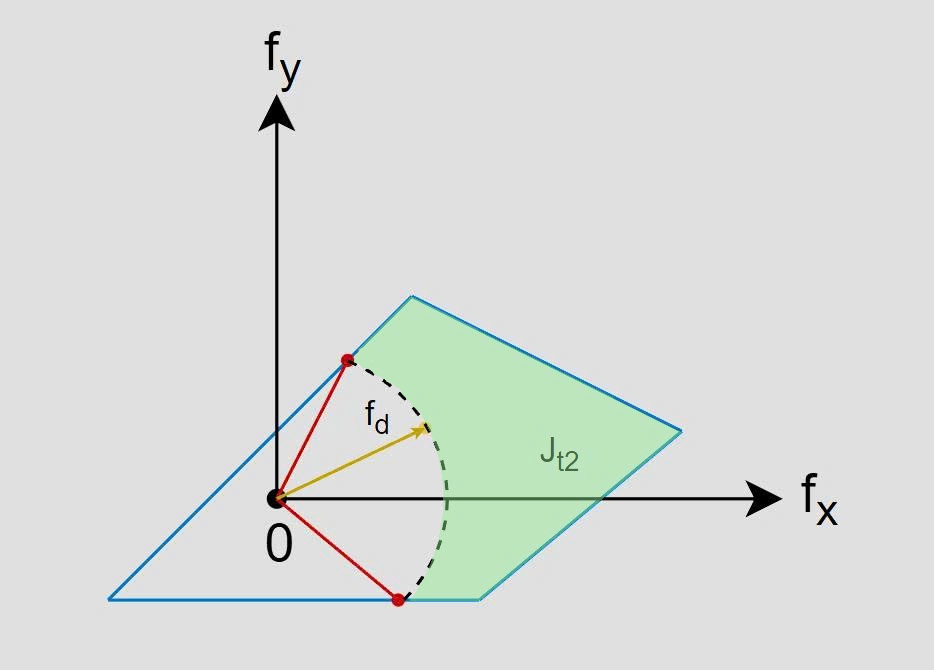
\includegraphics[scale=0.55]{chapter5/image/jt2.png}
    \caption{Độ ổn định tịnh tiến $J_\text{t2}$ đề xuất}
    \label{fig:metric2}
\end{figure}

Bài toán tối ưu thu được là phi lồi (non-convex) và không liên tục theo biến tối ưu $u$, do đó ta có thể dùng thuật toán ALPSO đã được đề cập ở trên để giải tìm nghiệm khả thi. Lúc này ta cần phải chuyển ràng buộc \ref{eq:op2} và \ref{eq:op3} thành các ràng buộc đẳng thức và bất đẳng thức để xây dựng hàm Lagrange tăng cường. Với ràng buộc \ref{eq:op3}, ta có thể viết lại như sau:
\begin{equation}
\label{eq:op1a}
g_{ij}(u) = d_{\min} - \mathrm{frD}(w_i, w_j) \;\le\; 0,
\qquad \forall i \neq j .
\end{equation}

Với ràng buộc \ref{eq:op2}, tương đương với $w_d$ nằm trong vùng không gian làm việc, ta có thể đánh giá thông qua $d_{\mathrm{signed}}(w_d, \mathcal{G}(w))$ là khoảng cách có dấu ngắn nhất từ $w_d$ đến biên của $\mathcal{G}(u)$.
\begin{equation}
d_{\mathrm{signed}}(w_d, \mathcal{G}(u))
=
\begin{cases}
> 0, & \text{nằm bên trong},\\[4pt]
= 0, & \text{tại biên},\\[4pt]
< 0, & \text{nằm ngoài}.
\end{cases}
\end{equation}

Khi đó ràng buộc \ref{eq:op2} có thể được biểu diễn lại là:
\begin{equation}
\label{eq:qu}
q(u)
= -\, d_{\mathrm{signed}}(w_d, \mathcal{G}(u))
\;\le\; 0
\end{equation}

Áp dụng công thức \ref{eq:al}, ta xây dựng hàm AL như sau:

\begin{equation}
\label{eq:ala}
\mathcal{L}(u,\lambda,\rho)
= J(u)
+ \sum_{i<j} \left[ \lambda_{ij}\, g_{ij}(u) + \frac{\rho}{2}\, \max\big(0,\; g_{ij}(u)\big)^{2} \right]
+ \lambda_{q}\, q(u)
+ \frac{\rho}{2}\, \max\big(0,\; q(u)\big)^{2}
\end{equation}

Khi sử dụng cơ chế phân tán và giải bằng DALPSO, để giảm mức độ truyền thông thì các robot chỉ chia sẻ thông tin $l_\text{best}$ và nhìn được $g_\text{best}$ toàn cục sử dụng global topology và cập nhật vị trí theo \ref{eq:vpso2}. Lời giải của bài toán tối ưu hàm \ref{eq:al} chính là cấu hình $u$ ổn định nhất để sinh ra wrench $w_d$ lên trọng tâm của vật. Bài toán tối ưu này có thể được chạy liên tục trong quá trình hoạt động của hệ thống, song song với việc lên chiến thuật đẩy vật. Lời giải mới nhất liên tục được lưu lại trong quá trình đẩy, và chỉ được sử dụng cho cơ chế chuyển đổi đội hình khi có hệ thống có kích hoạt. Điều kiện kích hoạt là khi có sự thay đổi trong đầu vào của hệ thống, như thay đổi số robot $n$ tham gia nhiệm vụ, và quan trọng hơn là khi mà ràng buộc \ref{eq:op2} bị vi phạm, tức là lúc này cấu hình hiện tại không còn có khả năng sinh ra $w_d$.


\section{Lên chiến thuật đẩy}
Việc lên chiến thuật đẩy có thể hiểu là việc tìm một bộ lực $f_r = [f_1 \ldots f_n]$ với $f_i \in R, i \in R$ thỏa mãn $w_d = w_e = G(u)\,f_r$. Như đã trình bày ở mục \ref{subsec:qp0}, việc nghịch đảo một cách đơn thuần mang theo rất nhiều rủi ro khi có vô số nghiệm thỏa mãn, cũng như nghiệm có khả năng vi phạm ràng buộc về mặt vật lý. Cách tiếp cận đúng đắn đó là xây dựng và giải một bài toán tối ưu theo \ref{eq:forceop}. Dựa theo nghiên cứu \cite{Rosenfelder2024}, bài toán sẽ được xây dựng ưới dạng một bài toán quy hoạch toàn phương (Quadratic Programming - QP). 
\subsection{Làm mềm ràng buộc}
Việc yêu cầu tác dụng chính xác $w_d$ có thể tồn tại một vài hạn chế, ví dụ trong trường hợp $w_d$ không nằm trong nhưng gần không gian làm việc $\mathcal{G}(u)$. Trong trường hợp đó, thay vì phải xây dựng lại cấu hình mới, điều kiện \ref{eq:op2} có thể được làm mềm, tức là không còn yêu cầu nghiệm phải thỏa mãn bằng đẳng thức một cách chính xác để dễ giải hơn. Nói cách khác là ta chấp nhận sai số trong một lân cận nhất định của $w_d$.
\begin{figure}[H]
    \centering
    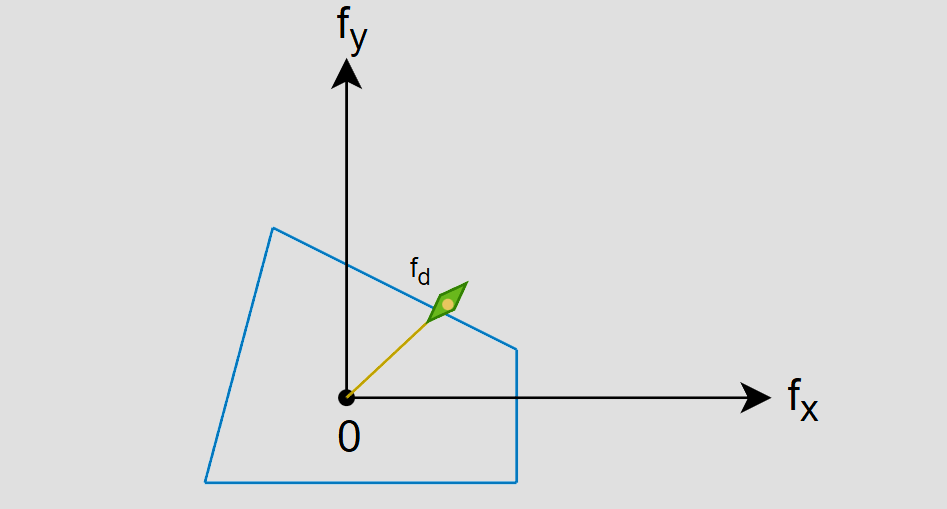
\includegraphics[scale=0.45]{chapter5/image/soft.png}
    \caption{Sai số chấp nhận theo dạng hình thoi}
    \label{fig:soft}
\end{figure}

Trong nghiên cứu \cite{Rosenfelder2024}, đối với lực tịnh tiến thì lân cận này được chọn là một hình thoi (rhombus) có tâm tại $f_d$ như hình (\ref{fig:soft}), trong đó một đường chéo của hình thoi trùng với hướng của $f_d$. Hai độ dài của hai đường chéo là hai tham số độc lập thể hiện mức độ nới lỏng điều kiện \ref{eq:op2}, trong đó thường đường chéo vuông góc với $f_d$ được chọn ngắn hơn so với đường chéo song song, vì hướng của lực tác dụng quan trọng hơn độ lớn tuyệt đối do hiện tượng ma sát và trượt, ta cũng có thể xây dựng cho chiều mô men xoay theo cách tương tự.
\subsection{Xây dựng bài toán quy hoạch toàn phương}
Bài toán tối ưu lực đẩy được mô hình hóa dưới dạng một bài toán quy hoạch toàn phương - QP, với hàm mục tiêu được thiết kế với các tiêu chí khác để có được lực $f_r$ như mong muốn dưới dạng:
\begin{subequations}
\label{eq:qp_force}
\begin{align}
\min_{f_r \in \mathcal{F}} \quad 
& \|G(u) f_r - w_d\|_{Q}^{2}
  + \|f_r - f_{\mathrm{set}}\|_{R}^{2}
  - \tilde{q}\, f_r^\top G(u)^\top w_d
\tag{\ref{eq:qp_force}a}
\\[6pt]
\label{eq:rhom}
\text{s.t.} \quad 
& C_\diamond \, G(u) f_r \le d_\diamond
\tag{\ref{eq:qp_force}b},
\end{align}
\end{subequations}
trong đó:
\begin{itemize}
    \item $\|G(u) f_r - s f_d\|$: Còn thể viết lại thành $\|w_e - w_d\|$ theo \ref{eq:we}, là hạng tử đo độ sai lệch giữa wrench tổng mà các robot đang tạo ra $w_e$ và wrench mong muốn $w_d$. Là thành phần quan trọng nhất, hướng tổng hợp lực và mô men sinh đến wrench mong muốn.
    \item $\|f_r - f_{\mathrm{set}}\|$: Hạng tử này giữ cho lực từng robot gần với giá trị đặt $f_{\mathrm{set}}$ mong muốn, tránh việc robot thay đổi lực quá đột ngột, giúp giữ lực trong một miền hoạt động an toàn.
    \item $f_r^\top G(u)^\top w_d$: Còn có thể viết lại thành $w_e^T w_d$, là tích vô hướng giữa wrench sinh ra và wrench mong muốn, đạt cực đại khi chúng cùng hướng. Hạng tử này giúp tổng wrench sinh ra cùng hướng với wrench mong muốn.
    \item $C_\diamond \, G(u) f_r \le d_\diamond$ là ràng buộc làm mềm (hình thoi) được đề cập ở trên.
    \item $Q \in R^{\text{3x3}} ,R \in R^{\text{nxn}} , \tilde{q} \in R_{\text{>0}}$ là cá ma trận hệ số dương.
\end{itemize}

Tương tự bài toán tìm đội hình \ref{eq:op}, việc thỏa mãn ràng buộc \ref{eq:rhom} là điều kiện tiên quyết để sinh được lực tổng thể, việc đạt cực tiểu của hàm mục tiêu có thể mang lại nghiệm đặc biệt mong muốn. Ma trận Hessian $H = 2(G^\top Q\, G + R)$ là bán dương (semi-positive), tuy nhiên ra có thể giả thiết $R > 0$ và do số hạng cuối là tuyến tính theo biến tối ưu, bài toán \ref{eq:qp_force} có nghiệm duy nhất. Mỗi robot tự giải ra bộ lực $f_r$ một cách độc lập với solver có sẵn, sau đó dựa vào vị trí tương ứng trong cấu hình đã thu được từ phần trên qua cơ chế thảo luận và phân nhiệm, robot tiến hành việc đẩy vật theo lực $f_i$ tương ứng mà nó tính toán ra.

